\documentclass[../thesis.tex]{subfiles}

\begin{document}
\chapter{System Overview}

\section{Concept}


\subsection{Monitoring}
The solar panel generates electricity and feed it into the converter after being measured by the current and voltage sensor. The converter converts the electricity from a higher voltage to a desired votlage, which can be measured again by the sensor and used to charge the battery. The sensing data consist of input current and voltage, and output current and voltage, which are fed into the microcontroller. The microcontroller has a 4G cellular modem which enables communication with the surrounding 4G cellular base station, and the internet access is provided by the gateway at the base station. That means, the sensing data can be be sent from the microcontroller to the server through the 4G cellular network. Once the sensing data reaches the server, the data is processed, store into the database, and send to the client such as a web application. The concept for monitoring is shown in the figure \ref{fig:concept1}.

\begin{figure}[!ht]
  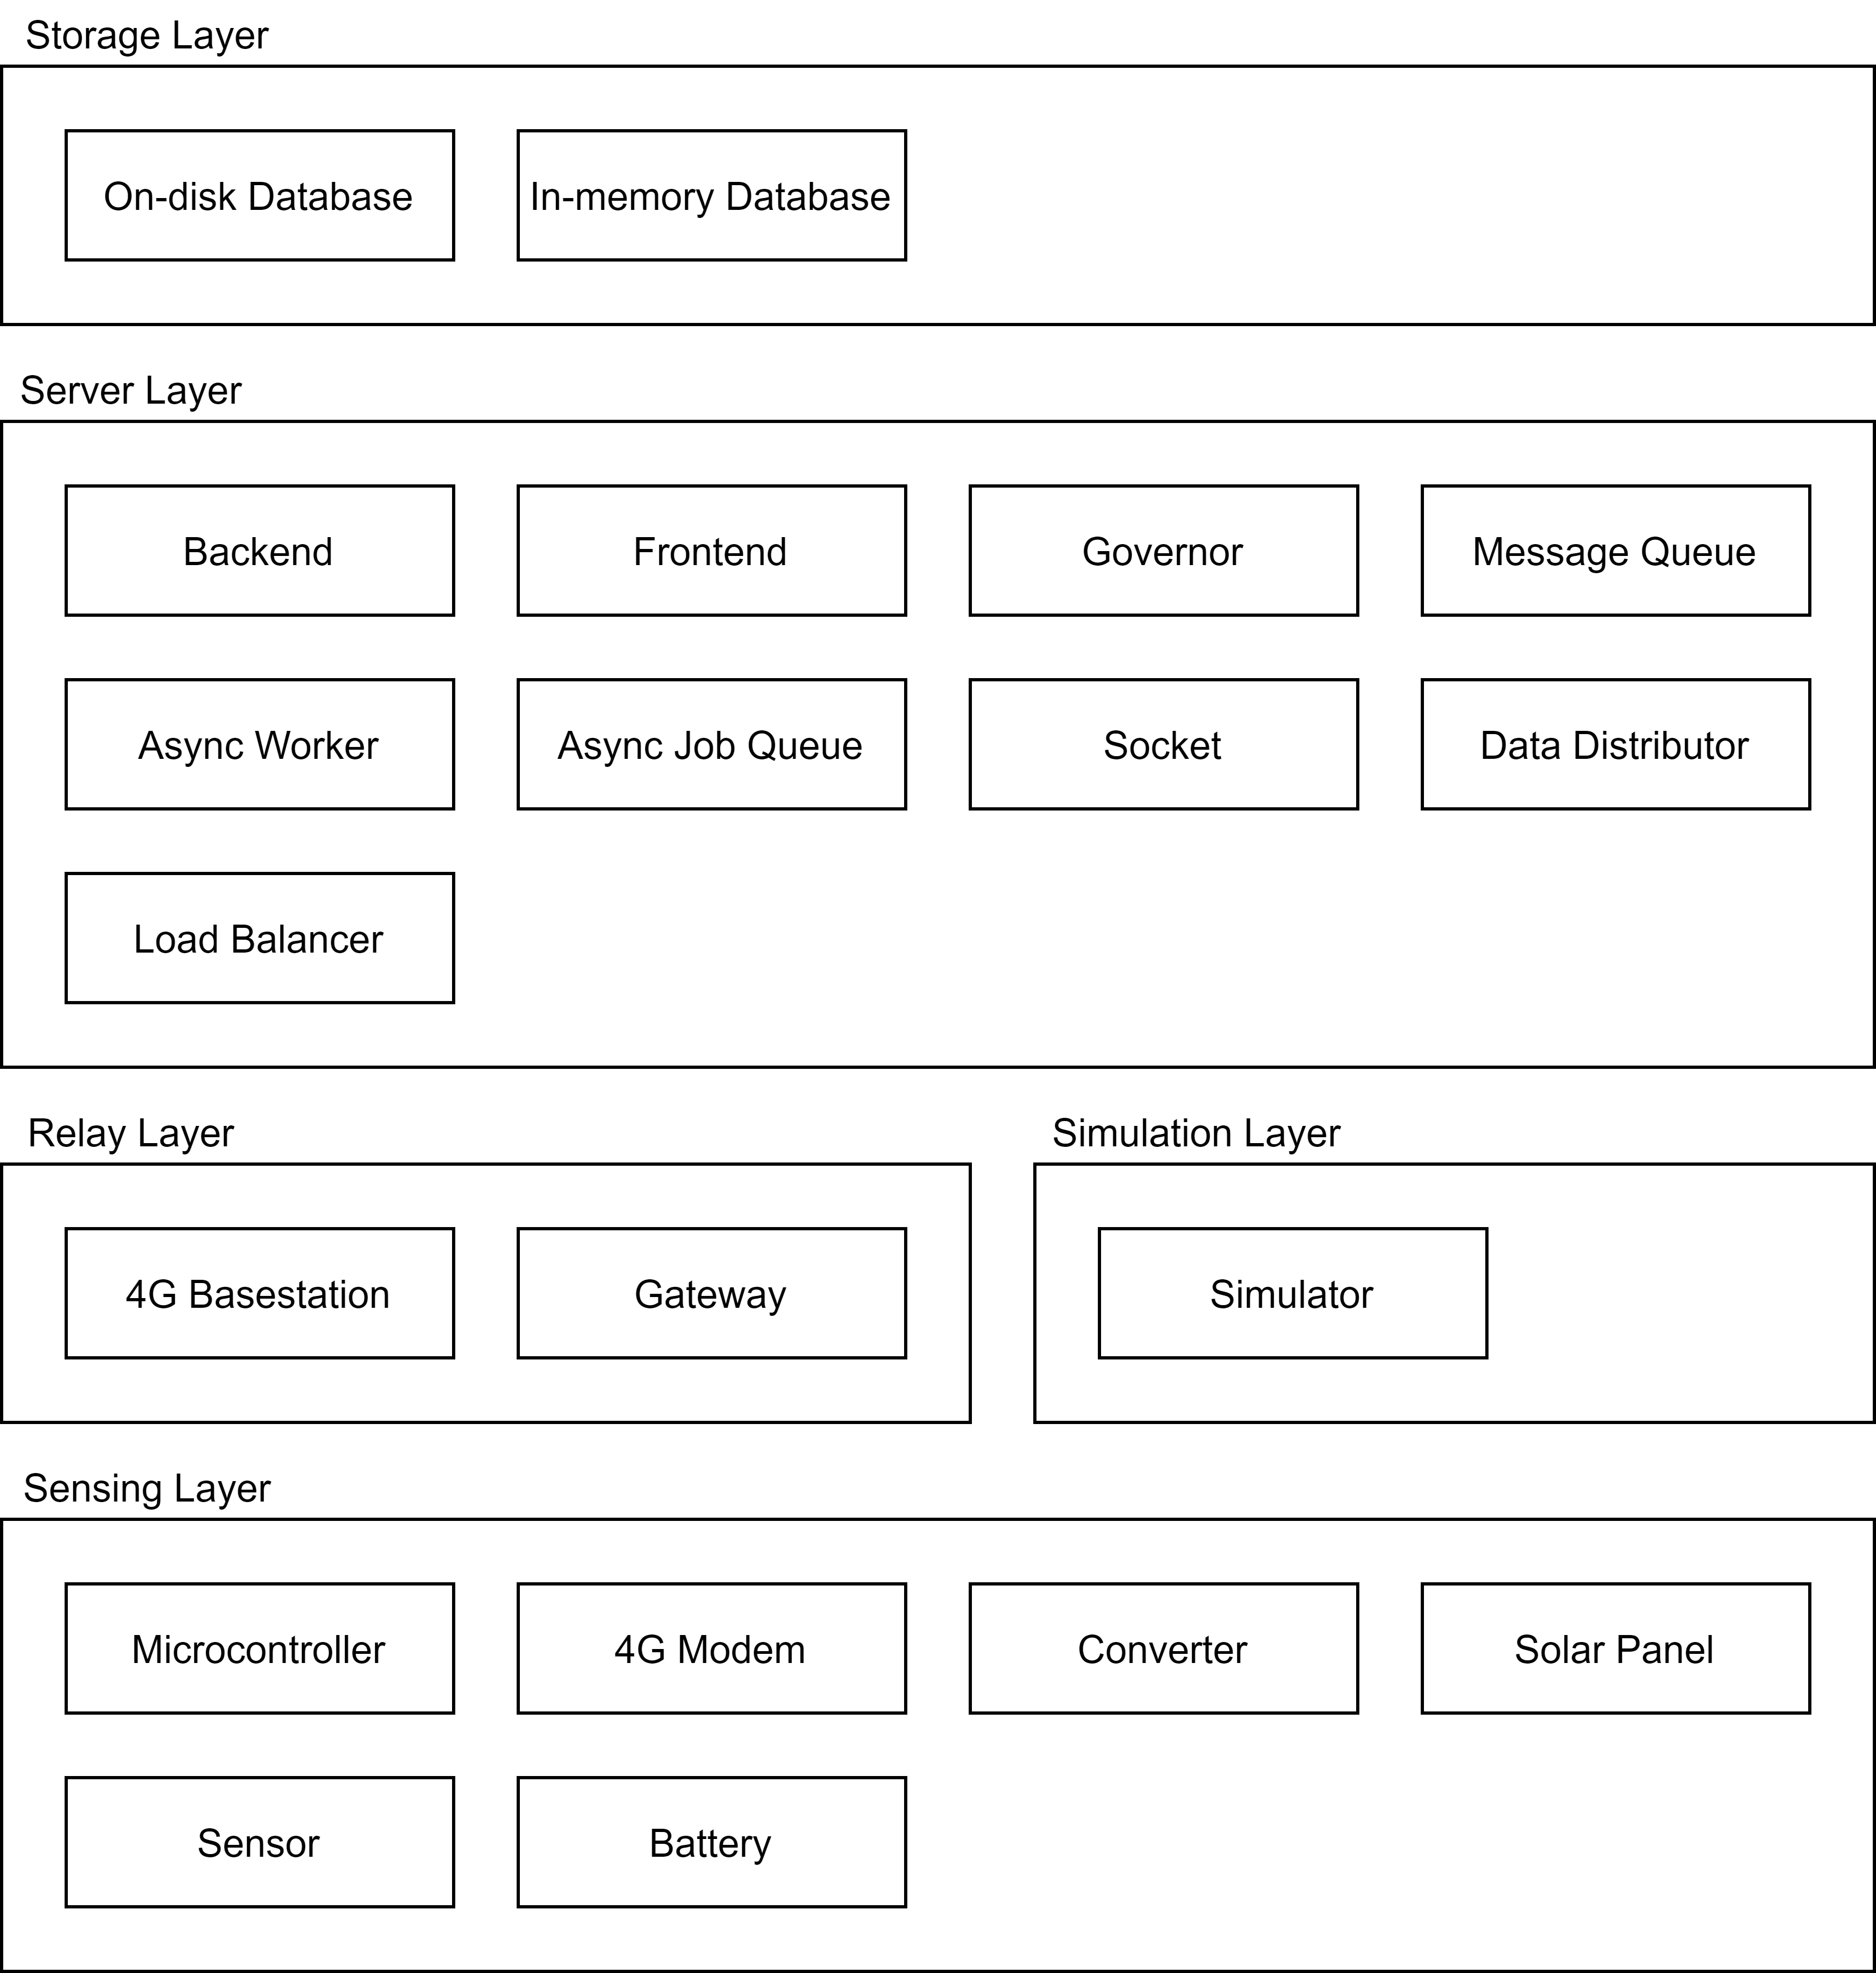
\includegraphics[width=\linewidth]{c3-concept-1.png}
  \caption{Concept of the proposed system for monitoring.}
  \label{fig:concept1}
\end{figure}


\newpage
\subsection{Controlling}
The lifecycle of a command begins at the client initiated by the user. The command can be anything from setting the output voltage, to shutting down the converter. Once initiated, the client contact the server to let it know a command had been issued, and the server store it in the database. 

On the other hand, the microcontroller performs periodic polling, that is, querying the server if there are new commands issued by the user every second. Similar to the monitoring, the query that is sent from the microcontroller to the server and the reply of the server that is consisting of a list of new commands are transmitted over the 4G cellular network. Finally, the commands are received by the microcontroller and the changes are applied to the converter. The concept for controlling is shown in the figure \ref{fig:concept3}.

\begin{figure}[!ht]
  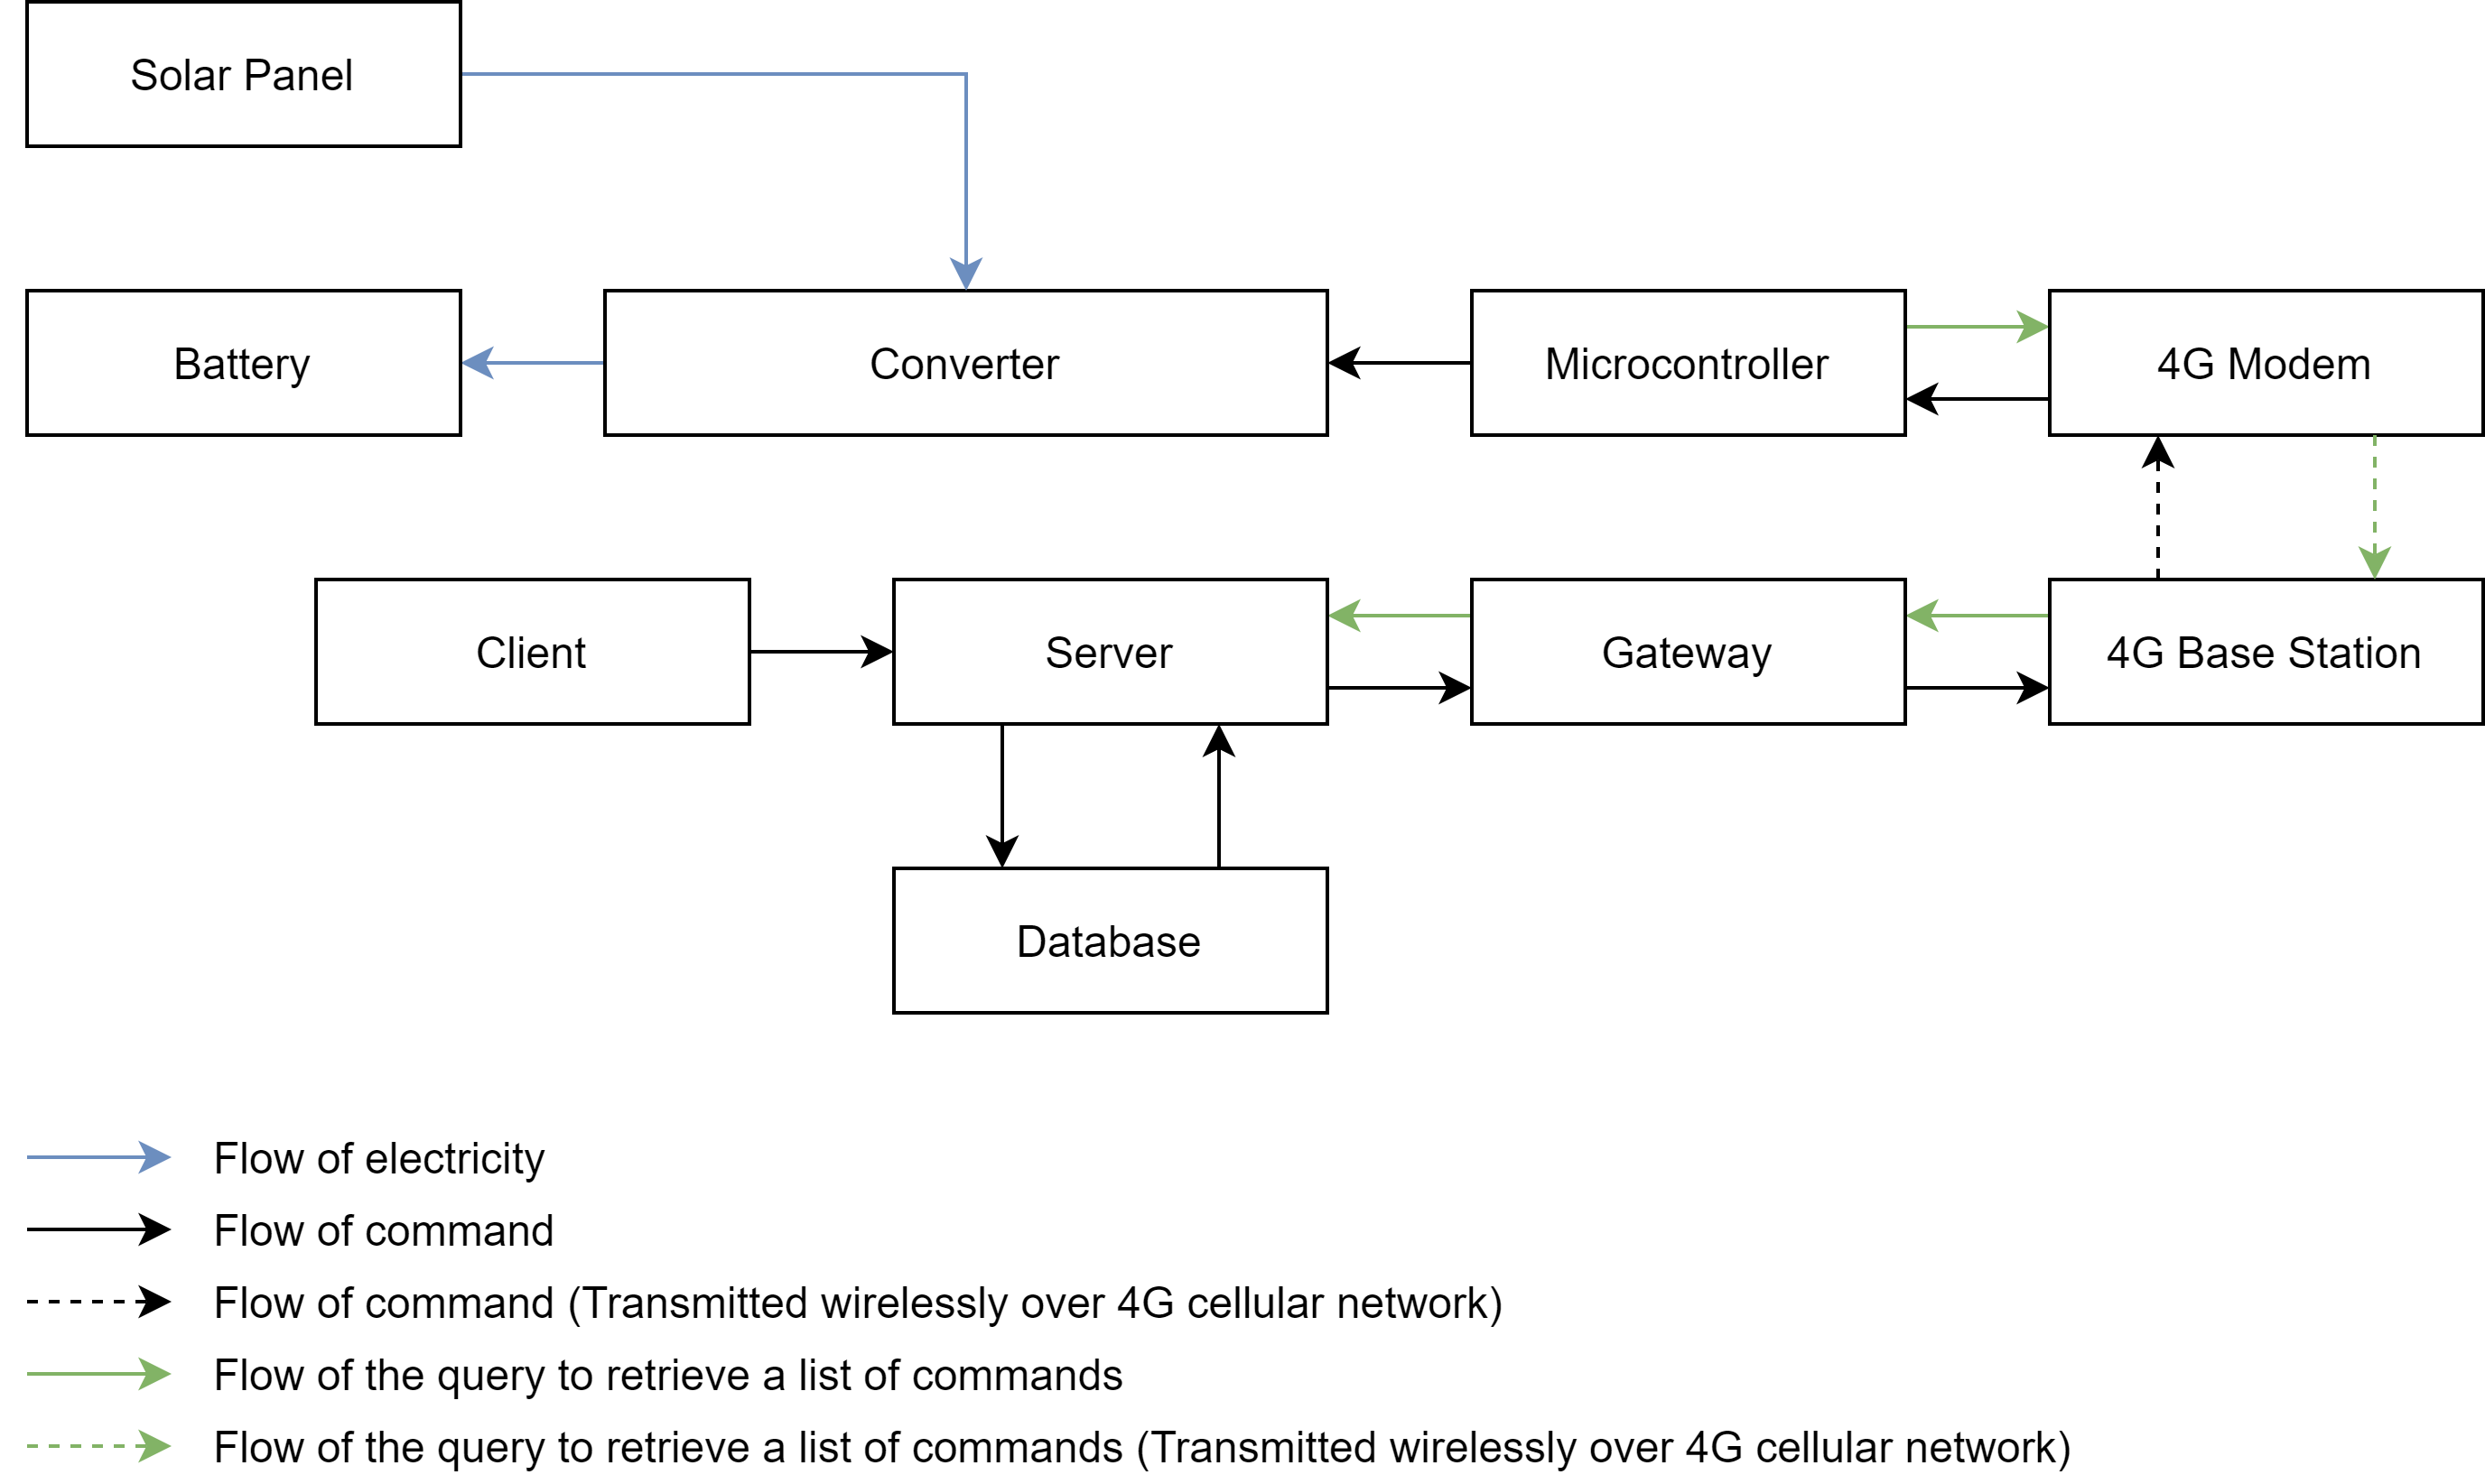
\includegraphics[width=\linewidth]{c3-concept-3.png}
  \caption{Concept of the proposed system for controlling.}
  \label{fig:concept3}
\end{figure}


\newpage
\section{Composition}

The proposed system is composed of five layers separated by responsibilities. They are:

\begin{itemize}
	\item Storage Layer
	\item Server Layer
	\item Relay Layer
	\item Simulation Layer
	\item Sensing Layer
\end{itemize}

The storage layer is responsible for storing the state of the server and sensing data received from the microcontrollers. The server layer is where the data processing logic, system monitoring, and data visualisation services are located. The relay layer contains the 4G infrastructures and providing internet access to 4G enabled devices. The sensing layer is responsible for measuring the data and control the generation of power. Lastly, the simulation layer is used to simulate the behaviours of the sensing layer for benchmarking purposes. Figure \ref{fig:concept2} shows the layers and the components within each layer.

\begin{figure}[!ht]
  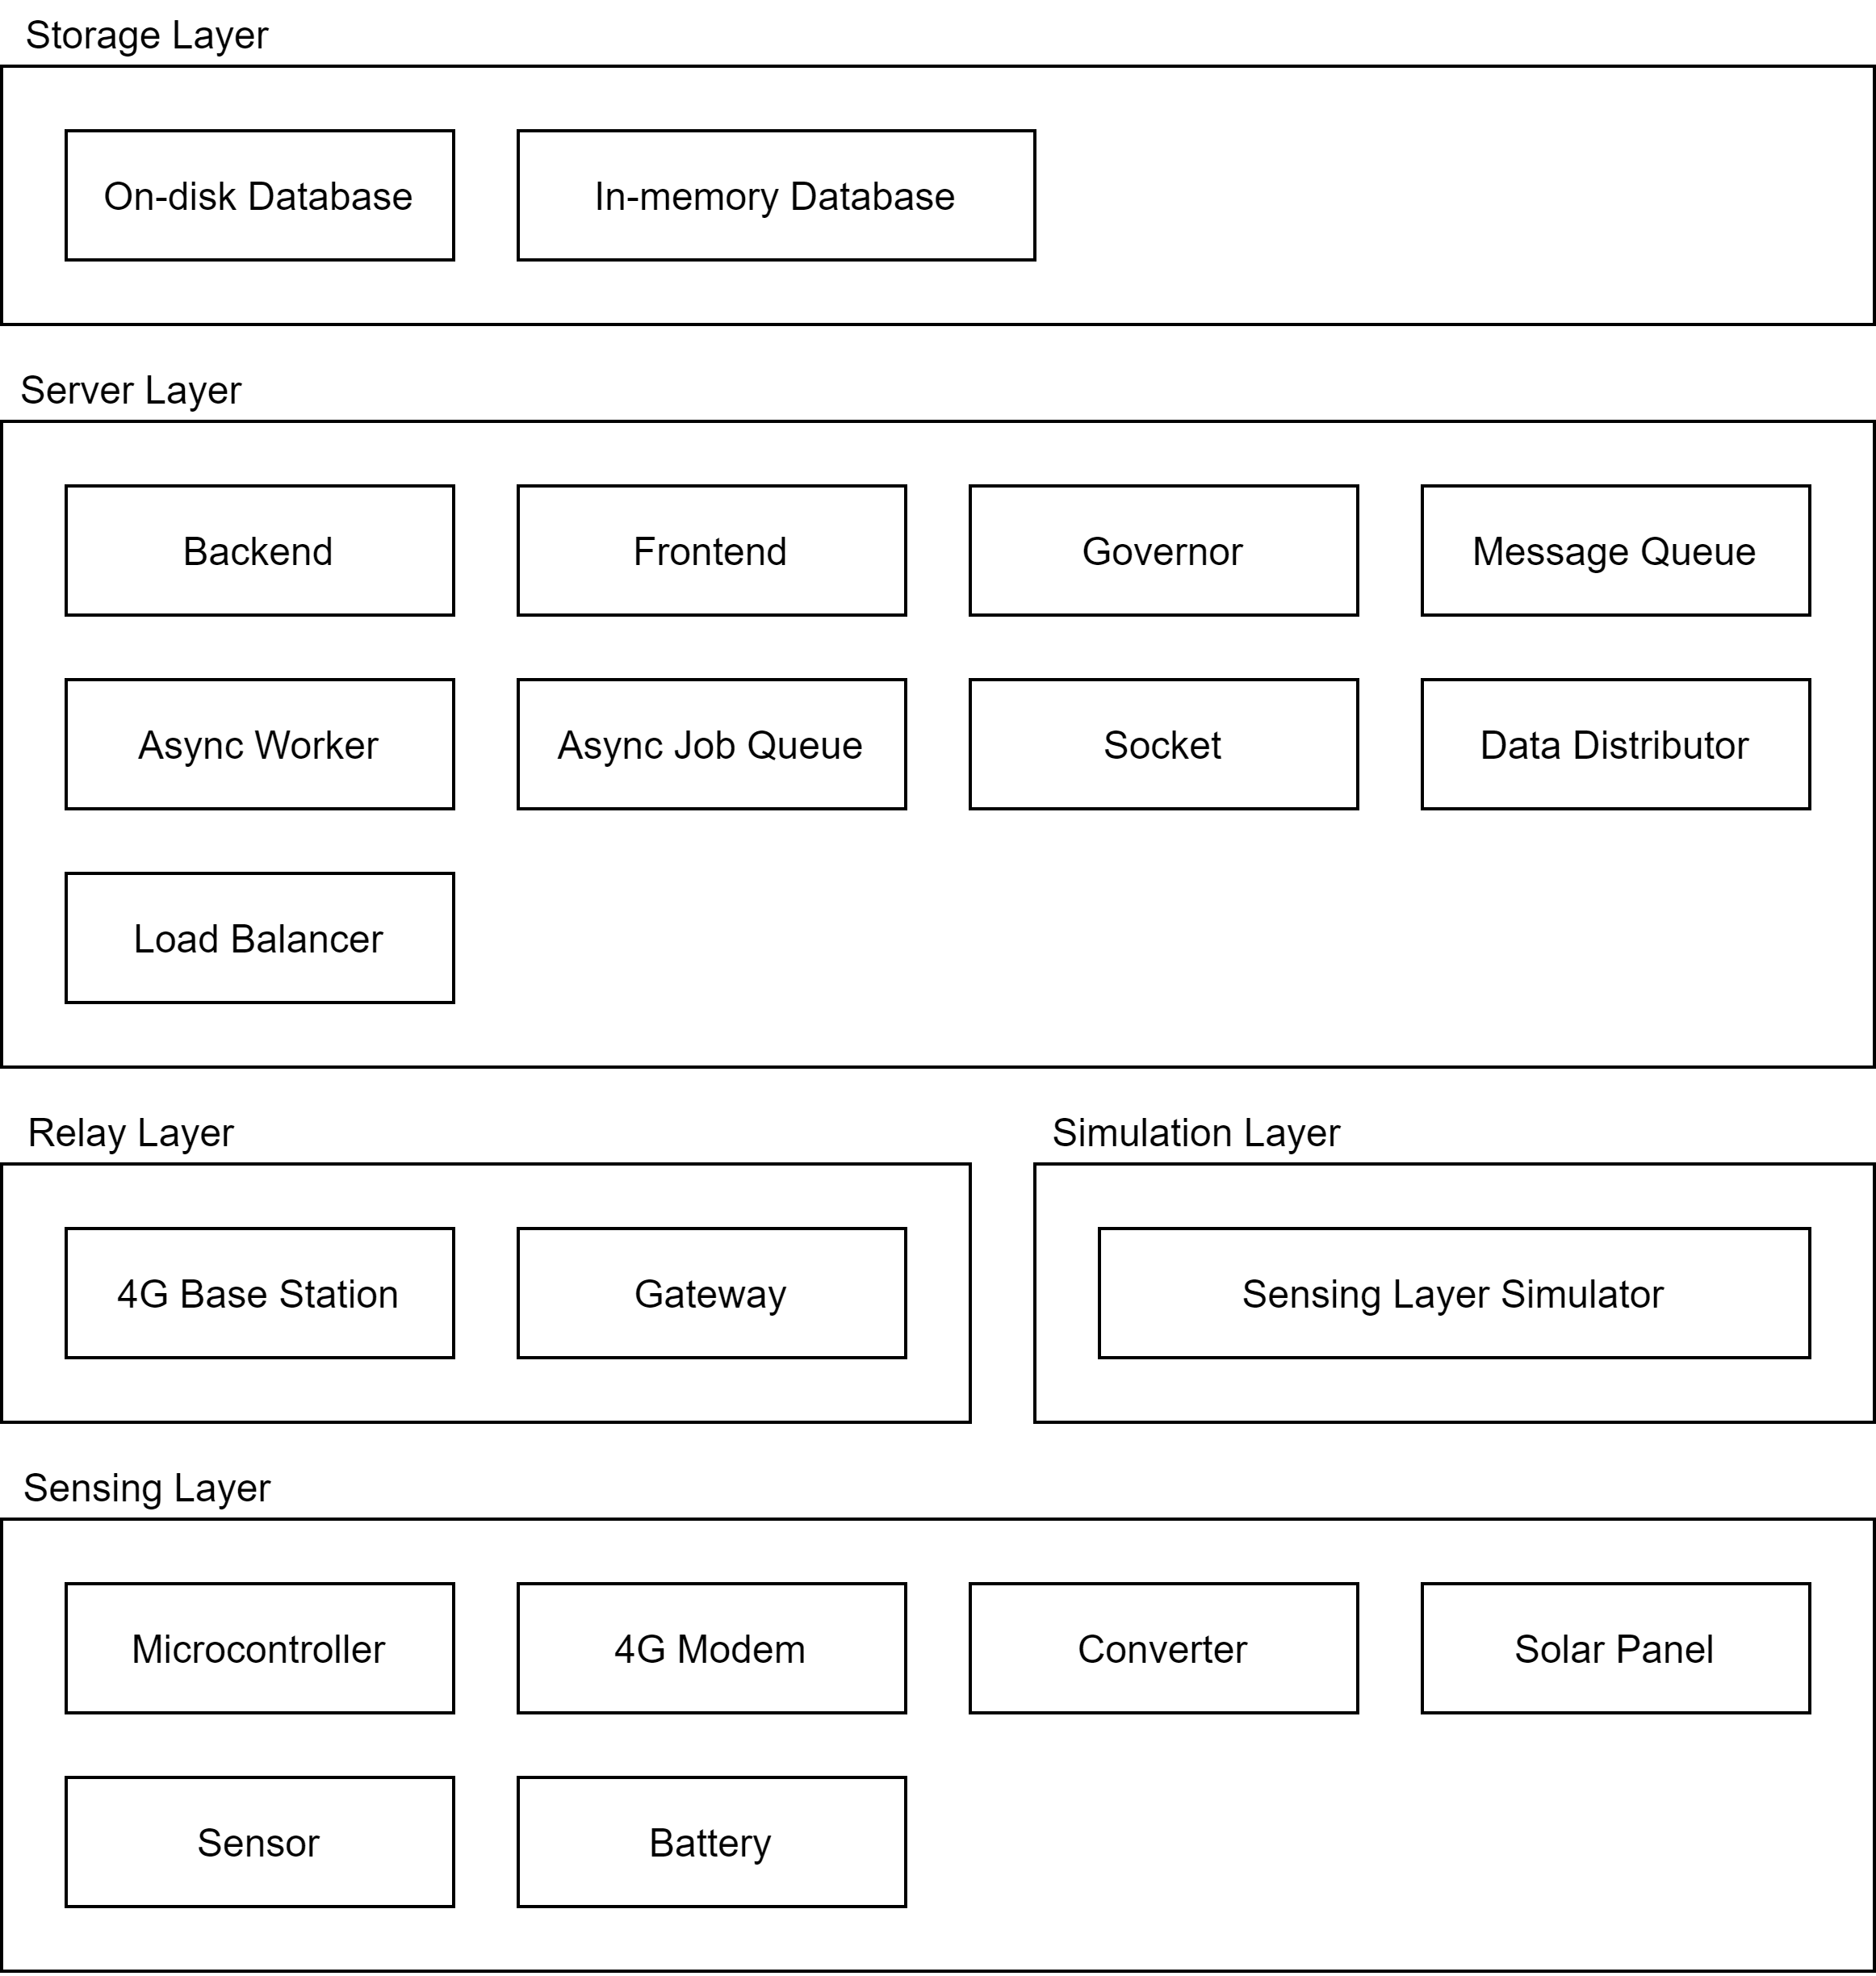
\includegraphics[width=\linewidth]{c3-concept-2.png}
  \caption{Layers and components of the proposed system.}
  \label{fig:concept2}
\end{figure}


\subsection{Storage layer}

There are two types of databases being used in the proposed system and each serves a different purpose. The two types are on-disk and in-memory. Figure \ref{fig:composition1} shows the technologies that are being used in this layer.

\begin{figure}[!ht]
  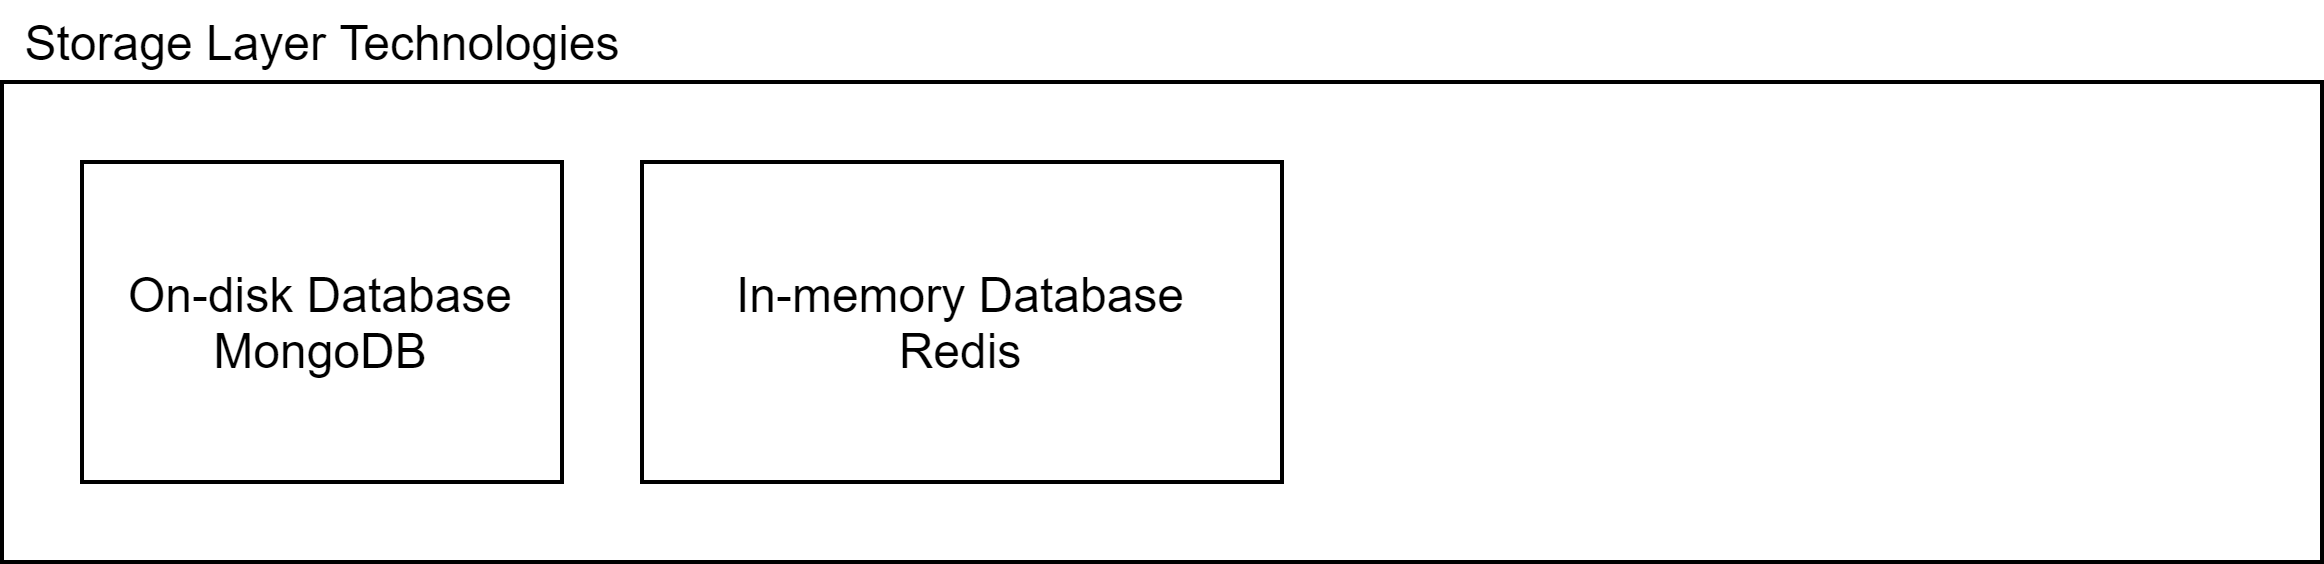
\includegraphics[width=\linewidth]{c3-composition-1.png}
  \caption{Technologies used in the storage layer.}
  \label{fig:composition1}
\end{figure}

\subsubsection{On-disk database}

The on-disk database used in the proposed system is MongoDB. The distinguishing characteristic of this type of database is the data that are stored in the database is persistant, which means the data remain intact even if the database is down due to failures. It is usually used to store a large amount of data reliably. The downside of using an on-disk database is the response time of querying and inserting data into the database can be very slow. The primary usage in the proposed system is storing the information, status, and sensing data of a device such as a solar panel persistently. 

\subsubsection{In-memory database}

The in-memory database employed in the proposed system is Redis. The goal for this type of database is not storing the data persistently but aiming to access, modify, and insert data as quick as possible. This advantage is the result of using the memory instead of the disk of the server, which is significantly faster. However, it also comes with the problem of having significantly smaller capacity, and the data is volatile. That is, the data is gone when the database is down and the data may be purged if the memory of the server is running low. This is primarily used to synchronise the state and sharing data between backend instances that are running on the same server. 

\subsection{Server Layer}

There are many technologies being used in the server layer to process sensing data, monitor the system, and provide data visualisation services, they are shown in the figure \ref{fig:composition2}.

\begin{figure}[!ht]
  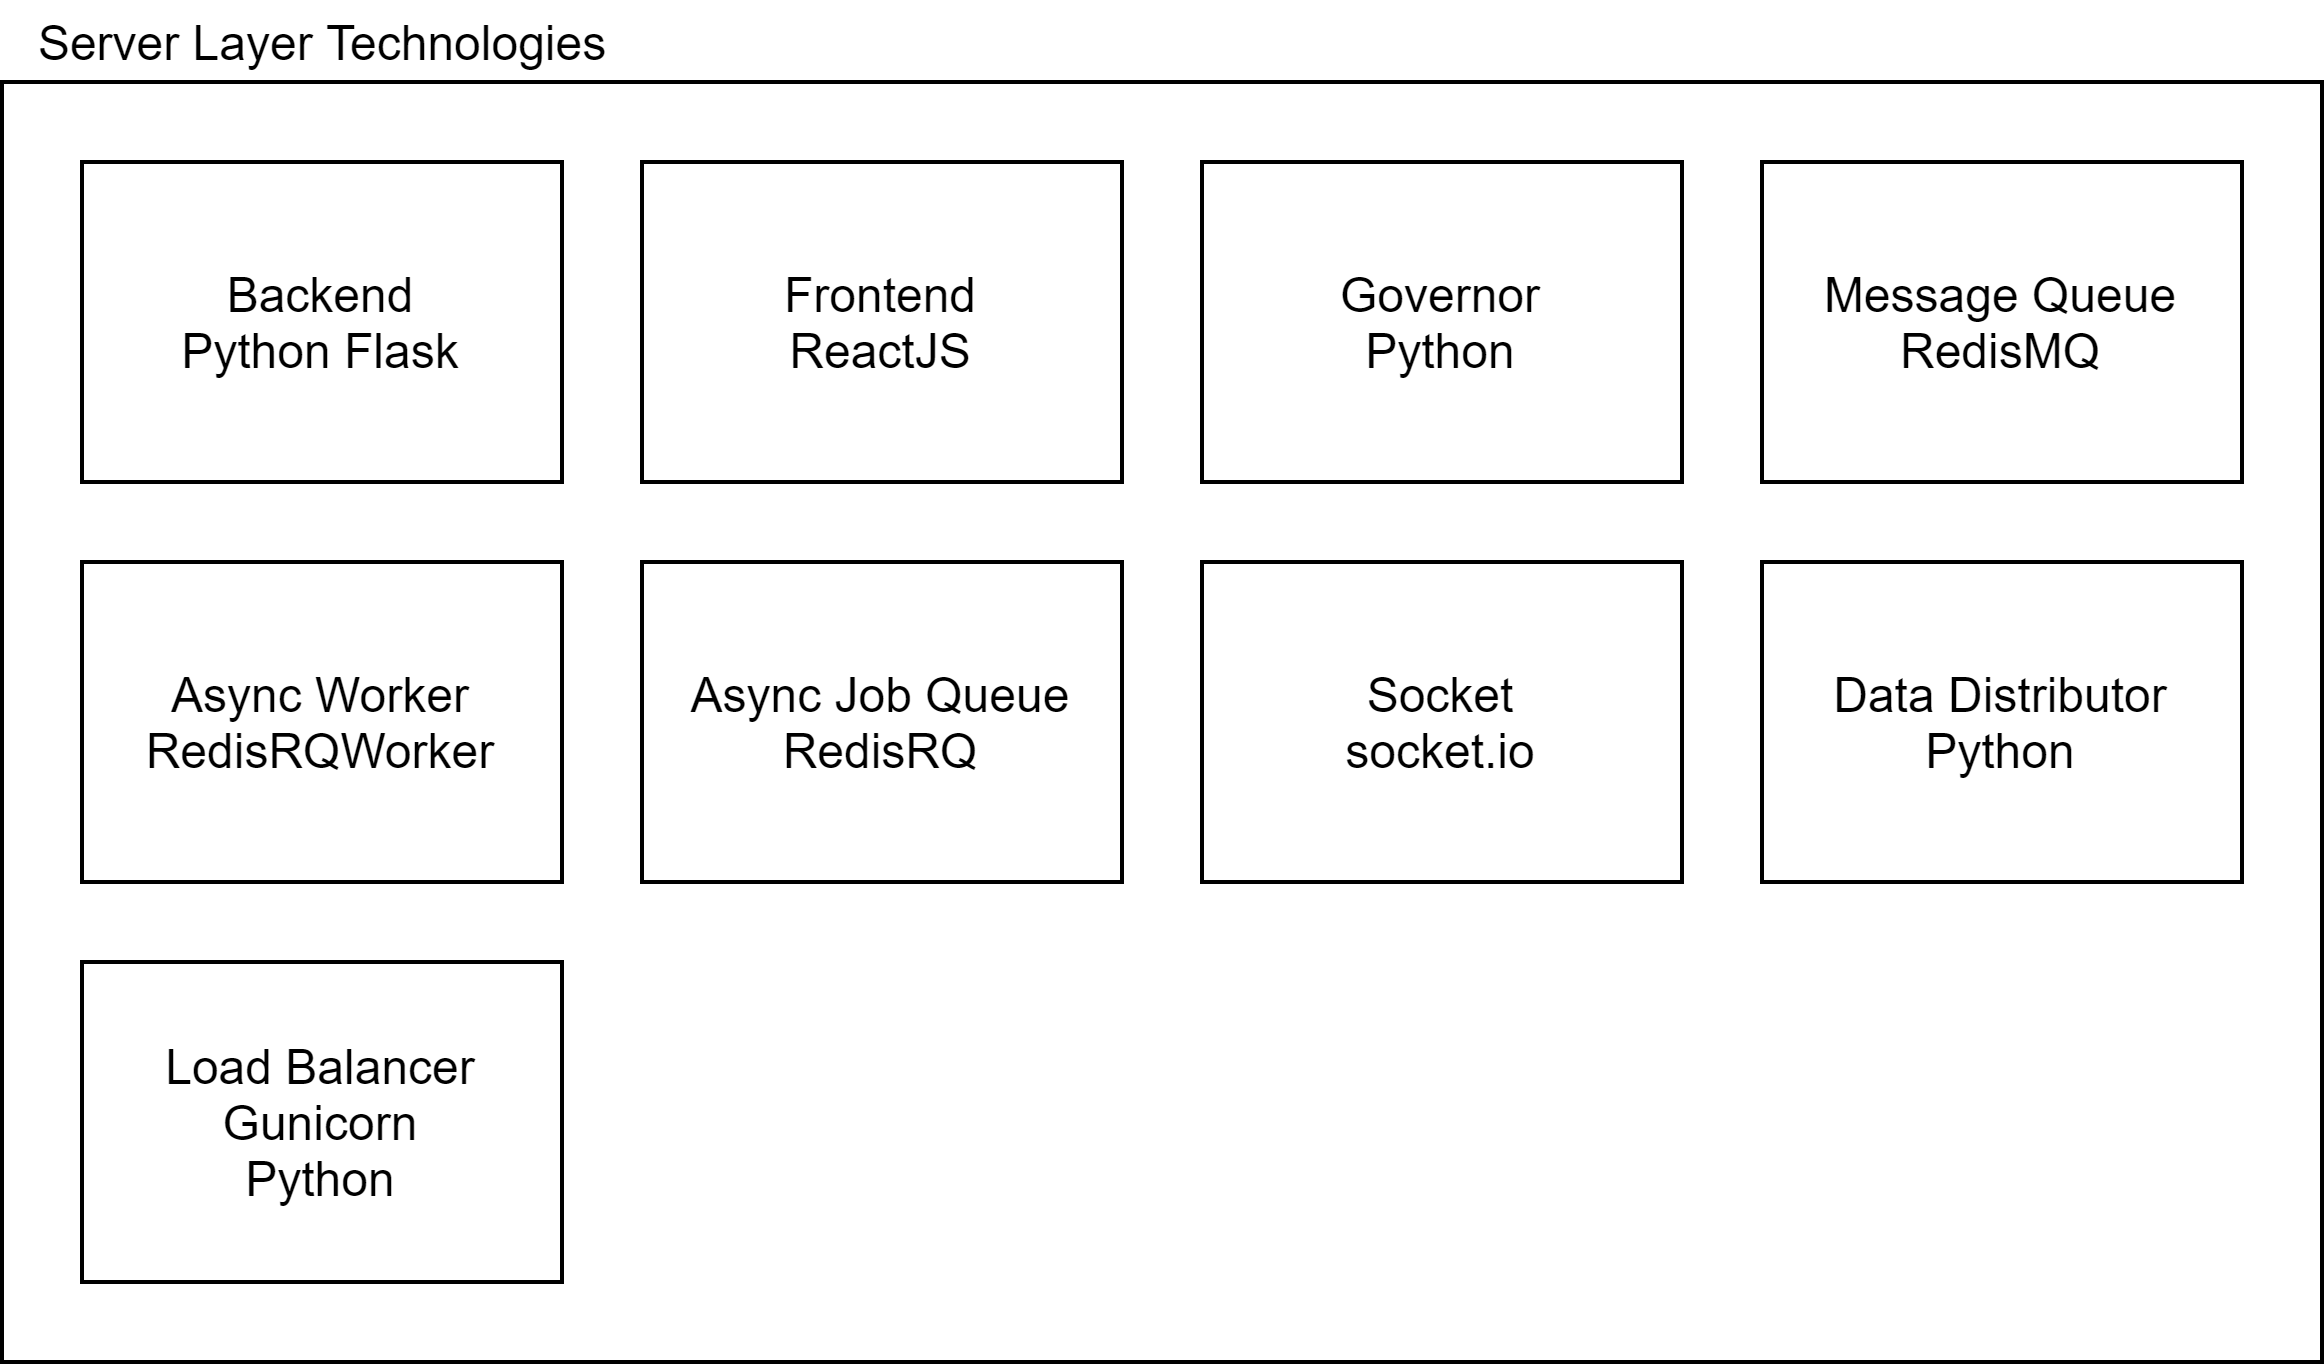
\includegraphics[width=\linewidth]{c3-composition-2.png}
  \caption{Technologies used in the server layer.}
  \label{fig:composition2}
\end{figure}


\subsubsection{Backend}

Backend is a stateless HTTP server powered by the Flask framework. Its responsibilities are:

\begin{itemize}
	\item Providing endpoints for microcontrollers to register itself, insert sensing data to the database, and retrieve issued commands.
	\item Providing endpoints for frontend to retrieve data for visualisation and notifying a command had been issued.
	\item Providing context-aware load balancing for frontend's real-time data visualisation. 
\end{itemize}

\subsubsection{Frontend}

Frontend is a web application built on top of the ReactJS framework and utilises socket.io real-time communication system. Its responsibilities are: 

\begin{itemize}
	\item Providing a pleasant and usable user interface.
	\item Providing a real-time data visualisation.
	\item Providing a control panel for issueing commands.
\end{itemize}

\subsubsection{Load balancer}

\subsubsection{Governor}

\subsubsection{Message queue}
\subsubsection{Async worker and job queue}

\subsubsection{Socket}
\subsubsection{Data distributor}




\newpage
\section{Hardware}

asdfsadfasdfasdfasdf

\section{Software}

asdfsadfasdfasdfasdf

\section{Cost estimate}

asdfsadfasdfasdfasdf

\end{document}